%!TEX root = ../thesis.tex
%\input{commands.tex}
%*******************************************************************************
%****************************** Third Chapter **********************************
%*******************************************************************************
\chapter{Haplotype phasing consistency as a signal for physical linkage in scaffolding and assembly}

% **************************** Define Graphics Path **************************
\ifpdf
    \graphicspath{{Chapter4/Figs/Raster/}{Chapter4/Figs/PDF/}{Chapter4/Figs/}}
\else
    \graphicspath{{Chapter4/Figs/Vector/}{Chapter4/Figs/}}
\fi



\section{Background}
\par{
Reference genomes have enabled a range of genomic analysis by providing prior knowledge of the sequence 
and giving genomic context as well as a common coordinate system by which to compare multiple genomes \cite{1000genomes} \cite{GRCh38}. Assembling reference genomes is complicated by repetitive sequences, heterozygosity, and sequencing errors. As discussed in Chapter 3, when an assembly encounters inexact homologous sequences, it must determine which of these cases the sequence differences are due to. 
If the assembler cannot distinguish between heterozygosity and repeats, and if no reads span the homologous sequence into more unique regions, the contig must end
to avoid assembly distant regions or sequence from different chromosomes together. Historically reference genomes were created by large haploid bacterial artificial chromosomes (BACs) clone libraries \cite{human}. 
These methods overcame much of the problem of resolving repeats and heterozygosity because of their length allowing them to read through all but the longest segmental duplications and the fact that they are inherently haploid. However, because each of these BACs were sequenced with Sanger sequencing and assembled, they were still subject to problems in repeats longer than the Sanger reads that were close enough to one another to occur in the same BAC clone. But most importantly, these methods are far too costly to apply to many genomes. 
}

\par{
More recently the cost reductions of long read technologies \cite{pacbio} \cite{oxford}, and reduced error profiles through optimization of the circular consensus method \cite{ccs}\cite{HIFI}
as well as the emergence of other long range genetic information technologies \cite{10xlinked} \cite{HiC} \cite{bionano} 
have converged to make high quality, cost effective reference genomes. This has then resparked interest in assembly 
as well as large reference generation projects. Efforts have begun on the Earth Biogenome Project (EBP)\cite{EBGP}, a global project to sequence the entire diversity of multicellular eukaryotic life. In the UK, the Sanger Institute and partners have started to sequence 60,000 species from the British Isles in the Darwin Tree of Life (DToL) project. These projects aim to provide a scientific resource for the next generation of biological science, for environmental conservation, and to study evolution at a much broader and deeper scale than ever before. 
}

\par{
As discussed in Chapter 3, one of the primary remaining difficulties in assembling reference quality genomes is high levels of heterozygosity such as found in many of the non-model organisms included in the EBG and DToL projects. While Chapter 3 focused on going from a pool of individuals---and thus many haplotypes---to a single individual---and thus two haplotypes, this chapter focuses on the problems encountered with high levels of heterozygosity within an individual and the improvements that can be made computationally to both alleviate those problems as well as use the high levels of heterozygosity to our advantage. 
For these newer technologies mentioned above, there are now assembly algorithms that deal with each data type \cite{falcon} \cite{supernova} \cite{bionano_assembly} 
as well as combinations of multiple technologies \cite{genemyers} \cite{hybrid10x} \cite{hicscafffirst}\cite{hicassembly}. 
 These methods try to co-assemble both haplotypes arriving at a haploid consensus \cite{watchtower} \cite{canu} 
 or a diploid assembly \cite{falconPHASE} \cite{supernova} \cite{hifiasm}\cite{dipasm}, but heterozygosity still injects complexity and ambiguity on top of a haploid assembly process.
}

\par{
As mentioned in Chapter 3, one method for dealing with the problem of heterozygosity is inbreeding organisms to a point of low heterozygosity \cite{drosophila}, 
but this is not possible for all organisms. Trio-sga used pedigree sequencing information in the assembly algorithm \cite{trio-sga} 
but was built for short reads and does not work on long read data. Recently Koren et al. described trio binning which uses a mother-father-child trio to 
separate long reads into their haplotype of origin prior to haploid assembly \cite{triobinning}. 
While this method is very effective, creating such a cross would be infeasible for many species and costly for the vast number of reference genomes these projects intend to sequence. 
Another recent approach using the new highly accurate HIgh FIdelity (HIFI) ccs reads from PacBio along with homopolymer compression and other methods to reduce errors dramatically is to 
require nearly identical sequence similarity to extend the assembly graph \cite{HICANU}. This results in the haplotypes being b v separately in all but the few long stretches of homozygosity in 
a genome. They then run a haplotic purging software PurgeDups \cite{purgedups} to remove one of the haplotype assemblies. This has the downside of not matching the haplotypes to make comparisons, but that could be done 
fairly well as an additional analysis step. This method does not explicitly phase the haplotypes and may have long phase switches especially across long regions of homozygosity.
}

\par{
Despite the incredible advances made over the past several years in both sequencing technologies and assembly methods, we still cannot assemble whole chromosomes or chromosome arms with a 
single technology for most organisms. After assembly we are left with some level of fragmentation of chromosomes into contiguous sequences (contigs) which we wish to scaffold together. While the 
PacBio HIFI technology has many wonderful properties including continuous, highly accurate reads, it does not produce long enough reads to span many repeat or low sequence complexity regions in most genomes.
 10x Genomics linked read technology, however, will create barcode linked short reads across much longer molecules (50kb+) with some molecules reaching well over 250kb \cite{10xlinked}. Optical map technology in which the DNA is linearized and flourescent markers are attached to sequence specific loci via restriction digestion and optically inspected can give sparse data for pieces of DNA about as long as can be isolated with modern high molecular weight extraction methods\cite{opticalmaps1}. And high-throughput chromatin conformation capture sequencing (Hi-C) data creates links between sequences physically located close to one another. And while there will be cross-chromosomal links, the large majority of links are intra-chromosomal but can create links of almost any length \cite{3CHIC} \cite{HIC}. Each of these technologies have been used to break misassemblies in contigs and scaffold contigs\cite{scaff10x}\cite{opticalhuman}\cite{hicscafffirst}\cite{SALSA}\cite{GRAAL}\cite{instaGRAAL}. But some of these scaffolders have been known to introduce misassemblies \cite{hicscafffirst}. 
}


\par{
While high levels of heterozygosity make the assembly problem harder for traditional methods, haplotype phasing consistency (reads containing multiple heterozygous alleles segregate into two---if diploid---groups according to which alleles they have) can be used as a signal of physical linkage in both assembly and scaffolding and as a method to differentiate inexact repeats from haplotype differences. While the conventional thinking is that heterozygosity makes these problems more difficult, we turn this around and use the phasing consistent property of heterozygous sites as a powerful way to simplify and add statistical power to them. In this chapter we present a toolkit for phasing, phasing aware assembly, and phasing aware scaffolding called phasstools (PHasing and ASSembly tools). It is made up of a number of github repositories with a master repository to give a unified command line interface. The code is open source and available at https://github.com/wheaton5/phasstools and the submodule repositories which are linked from the main repository. The use cases are reference based and fully de novo haplotype phasing, assembly based phasing aware scaffolding, and phasing aware assembly. While I will show results from the phasing aware assembly, these are preliminary and not without problems, which I will discuss. For that reason, I will first address the steps required to use phasing consistency for highly accurate assembly scaffolding. First I will outline phasing consistency, then introduce heterozygous single nucleotide polymorphism (SNP) kmer pairs as a mechanism for fully de novo haplotype phasing. Next I introduce an algorithm for de novo haplotype phasing using sparse \textit{Bernoulli} mixture model clustering---an algorithm very similar to the clustering algorithm used in Chapter 2. Afterwards I describe a phasing algorithm based on a given assembly to then be used for phasing aware scaffolding.
}


\section{Phasing aware scaffolding of an existing assembly: phasst scaff}

\par{
Our goal is to use the phasing consistency of Hi-C reads and optionally linked reads that cover heterozygous sequence on two contigs. First we must find those heterozygous sites. Then we can define phasing consistency of those sites.
}


\subsection{Paired heterozygous SNP kmers}
\par{
In the case of scaffolding an existing assembly, we could map the reads to the assembly and call variants to find heterozygous sites as is the common workflow for resequencing efforts. In an effort to be unbiased by the 
assembly, and to be general to a de novo assembly process, we will use paired SNP kmers---kmers that vary only in the middle base and that have counts that are roughly half of the homozygous kmer counts. We generate the 
kmer count spectra with a fast disk backed kmer counter KMC \cite{kmc}\cite{kmc2}\cite{kmc3}. Figure \ref{figure:kmc} shows an example kmer count histogram. 
}

\begin{figure}[htbp!]

\caption{Kmer count spectra and heterozygous paired kmers}
\label{figure:kmc}
\begin{centering}
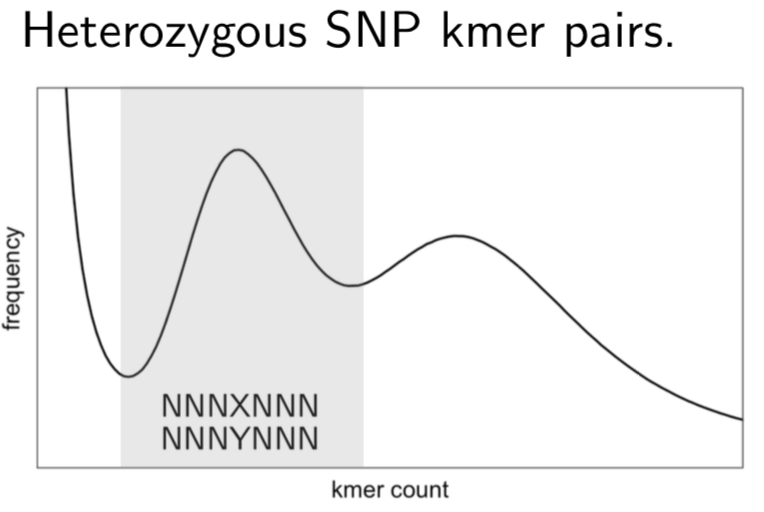
\includegraphics[width=0.65\textwidth]{kmc.png}
\par{An example of kmer count spectra showing error kmers on the left, heterozygous kmers in the first peak and homozygous kmers in the next peak.}
\end{centering}
\end{figure}

\par{
We then use the heterozygous range of the kmer spectra with code from purge dups, a tool for removing sequences from assemblies when multiple haplotypes were assembled separately\cite{purgedups}. The kmers are then dumped in alphabetical order and we search for pairs of kmers which vary in only the middle base and fall into the heterozygous counts range. We give a further restriction that the sum of the counts of the kmers with the other two possible bases in the middle are not high as sequences with very high repeat count can produce, through sequencing error or mutations, two kmers in these counts range with the middle base altered. It should also be noted, that while I generally refer to these kmer pairs as heterozygous kmer pairs, they may also represent paralogous kmer pairs. We will use the phasing consistency of these kmer pairs with each other to determine if they are more likely to be from heterozygosity or paralogous sequences. Each produces a characteristic pattern in the kmer consistency counts.
}

\subsection{Read data kmer information}
\par{
We will use the kmers in the reads to determine if heterozygous paired kmers are phasing consistent with other paired kmers. So we go through the reads of each long range genetic information including HiC, PacBio, linked reads, and nanopore and store the position and ID of each paired kmer on the reads. We then store this on disk in a custom binary format for later use. Of note here is that the linked read technology may have multiple molecules per barcode whereas in other technologies, reads represent single physically linked molecules. Richard Durbin has developed a method to \textit{de novo} assign reads from barcodes to molecule groups using shared kmers across barcode sets to cluster reads into their molecules of origin. In this work, we choose not to use this as it is unpublished and not extensively tested. Instead, we use the distance on the assembly contigs to determine which reads came from which barcode. With the recommended DNA input, high molecular weight (HMW) extraction sizes, and number of partitions, we expect the poisson loading to result in a mean of roughly ten molecules per barcode. Because the total amount of DNA per partition is a small percentage of the total genome sizes we work with, the chances of a partition having molecules which arose from nearby or overlapping locations is rare. Thus we can deduce that reads from a barcode which map close to one another on a reference or assembly arose from the same HMW molecule. While this is not fully \textit{de novo}, it is highly unlikely to cause a false inference because a chimeric misassembly causing incorrect linked read molecule inference would not result in a phasing consistent signal.
}

\begin{figure}[htbp!]

\caption{Identify paired kmer location in long range genetic data}
\label{figure:techs}
\begin{centering}
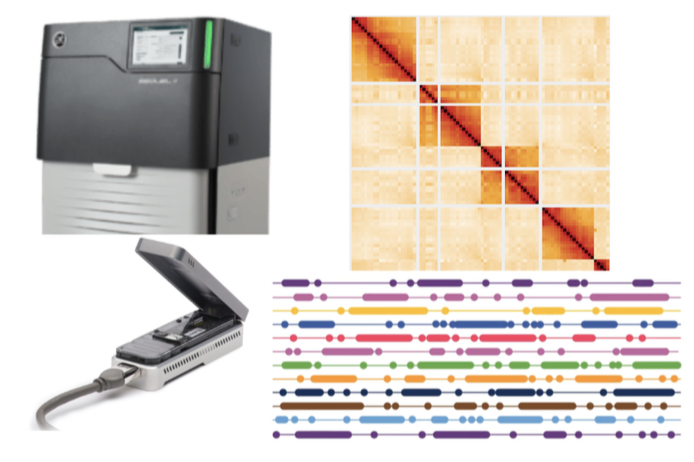
\includegraphics[width=0.65\textwidth]{techs.png}
\par{Different data types used. Top left: PacBio, Top right: Hi-C, Bottom left: nanopore, Bottom right: Linked reads}
\end{centering}
\end{figure}

\subsection{Pairwise haplotype phasing consistency}
\par{
For each kmer pair, we refer to one as the reference allele and one as the alternate allele arbitrarily without loss of generality. 
}


\begin{figure}[htbp!]
\caption{Pairwise phasing consistency counts}\label{figure:consistency}
\centering
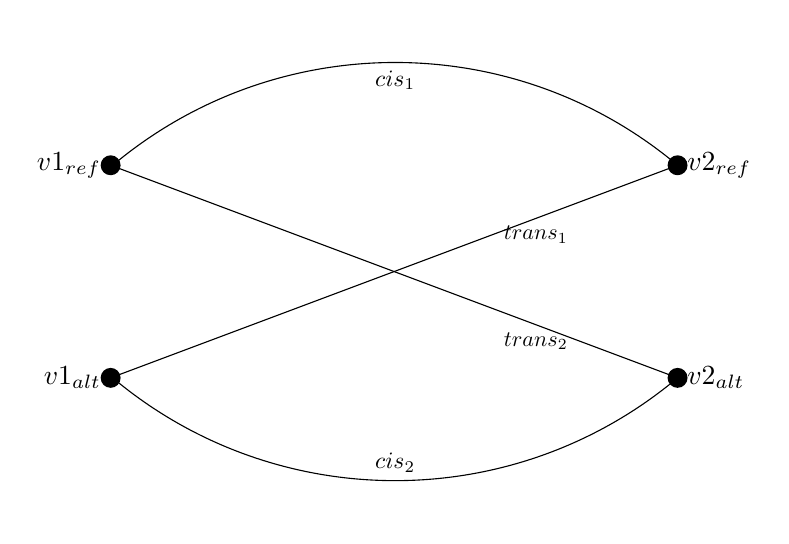
\begin{tikzpicture}[scale=1.8]
\def\xoffset{0}
\def\yoffset{0}
\def\titley{1.2}
\def\panellength{5}
\def\titlescale{1}
 \def\subtitlescale{0.7}
 \node[anchor=east] at (0 + \xoffset,2 + \yoffset) {$v1_{alt}$};
\draw (4 + \xoffset,2 + \yoffset) arc (-50:-130:3.1) node[midway,above, scale=0.85] {$cis_2$};
\fill (0 + \xoffset ,2 + \yoffset) circle[radius=2pt];
\node[anchor=west] at (4 + \xoffset,2 + \yoffset) {$v2_{alt}$};
\fill (4 + \xoffset,2 + \yoffset) circle[radius=2pt];
\node[anchor=east] at (0 + \xoffset,3.5 + \yoffset) {$v1_{ref}$};
\fill (0 + \xoffset,3.5 + \yoffset) circle[radius=2pt];
\draw (4 + \xoffset,3.5 + \yoffset) arc (50:130:3.1) node[midway,below, scale=0.85]{$cis_1$};
\draw (4 + \xoffset ,3.5 + \yoffset) -- node[below, scale=0.8] {$trans_1$} (2 + \xoffset,2.75 + \yoffset) -- (0+ \xoffset,2 + \yoffset);
\draw (4 + \xoffset,2 + \yoffset) -- node[below, scale=0.8] {$trans_2$} (2+ \xoffset,2.75 + \yoffset) -- (0+ \xoffset,3.5 + \yoffset);
\node[anchor=west] at (4+ \xoffset,3.5 + \yoffset) {$v2_{ref}$};
\fill (4+ \xoffset,3.5 + \yoffset) circle[radius=2pt];
\end{tikzpicture}
\par{
We denote one of each kmer pair as the reference or alternative arbitrarily. Molecules that have the sequences of one of the kmers from each of two kmer pairs will fall into one of four cases represented here by the four edges in this graph. We calculate the counts of molecules falling into each of these four categories. Phasing consistent heterozygous kmer pairs will have counts predominantly on both cis edges or both trans edges.
}
\end{figure}

\subsection{Multiple heterozygous site haplotype phasing consistency}



\subsection{de novo haplotype phasing}

\subsubsection{Sparse \textit{Bernoulli} mixture model clustering}


\cite{HICphasing} %place this somewhere





\section{Pedigree sample strategies}
As discussed already there are simple strategies for splitting long reads by haplotypes using short accurate reads from both parents. 
But for many species such as wild caught samples it may be difficult to obtain the paternal sample whereas it is possible to capture a 
fertilized female and grow her brood in isolation. For this case we propose to use three short read samples: one maternal sample, one sample 
from a single F1, and another sample from a pool of multiple F1 offspring. From these samples we can obtain distinguishing kmers or probabilistic 
distinguishing kmers for each haplotype of both the mother and father.

\begin{figure}[h!]
\caption{Pseudotrio}
\label{figure:pseudotrio}
\begin{centering}
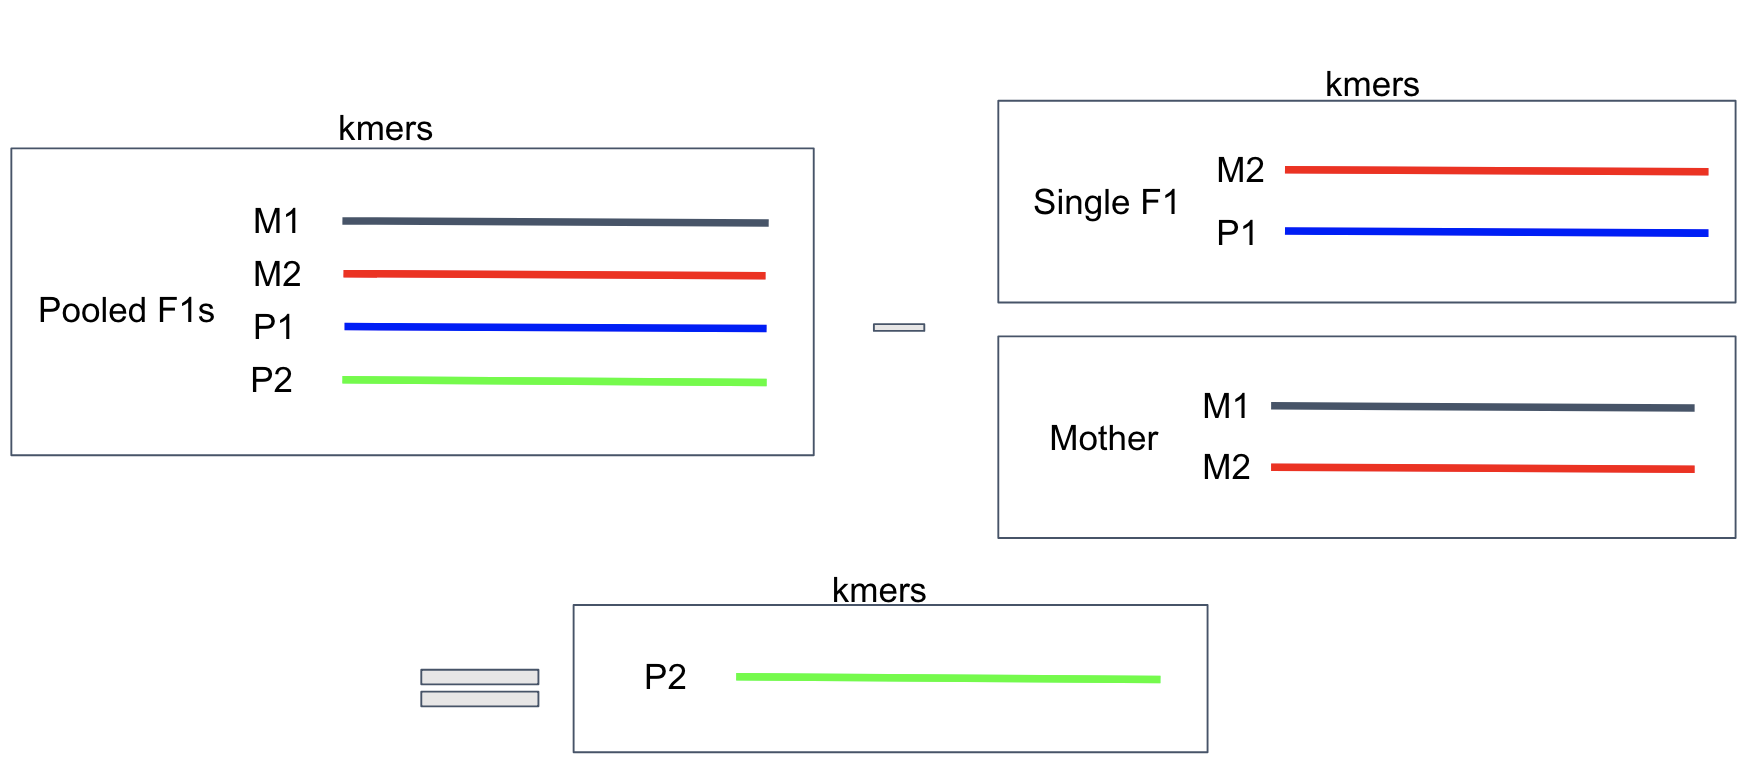
\includegraphics[width=\textwidth]{pseudotrio.png}
\end{centering}
\end{figure}

As shown in \ref{figure:pseudotrio} we can obtain distinguishing kmers for the P1 haplotype by set subtraction of kmers in the maternal and single F1 sample 
from the those in the pooled samples. In a similar way we can subtract kmers in the maternal sample from the single F1 sample to get probabilistic distinguishing 
kmers from the P2 haplotype. We say probabilistic distinguishing kmers because these kmers could also occur on the P1 haplotype as well. And in the same way 
we can get probabilistic distinguishing kmers for the M1 haplotype by subtracting kmers in the single F1 sample from those in the maternal sample. And finally we can obtain 
probabilistic distinguishing kmers for the M2 haplotype will be obtained by selecting kmers which are shared between the maternal and single F1 sample and occur at 
haploid counts in both samples. Once we have these distinguishing kmers we can use them to separate long reads by haplotype for libraries created from any of these samples. 
We have created software for collecting these distinguishing kmers \cite{distinguishing_kmers} which uses counting bloom filters to minimize memory usage 
and a mod based system allowing distribution of jobs to many worker nodes. And we also have software for binning long reads based on those 
distinguishing kmers \cite{long_read_binner}.


\section{Phasstools: phasing and assembly tools}
\subsection{Heterozygous kmer pairs and detection}
First we tackle the subject of identifying heterozygous variants in a reference-free manner. We will do this using a kmer approach, as many reference-free methods do. 
Many people have focused on identifying kmers which occur at roughly half counts in short read data \cite{KAT} and various software exists to count kmers \cite{jellyfish} 
and to model the mixture of expected distributions (errors, haploid, diploid, duplication kmers) \cite{genomescope}. Identifying heterozygous kmers in this way 
suffers from multiple problems from the perspective of de novo phasing. 1. Many of these identified as half counts will be either randomly high count error kmers or randomly low count 
homozygous kmers. 2. You end up with $K-1$ overlapping kmers for a given variant which is needlessly redundant information which will both slow down any phasing algorithm and 
likely break key independence assumptions. And 3. while you have heterozygous kmers, you don't know which kmers are alternative alleles of each other. 
We propose finding pairs of kmers which vary only in the center position which are also both roughly at half counts. These heterozgyous SNP kmers 
will be much more robust and have the benefit of knowing that one is the alternative allele of the other.
We have software for this purpose \cite{het_kmers} which uses counting bloom filters to minimize memory usage and a mod based method to 
distribute the work to many worker nodes.

\subsection{Phasing consistency}

\subsection{Data types and uses}


\subsection{Phasst phase: Reference or assembly based phasing}
\subsubsection{Sparse \textit{Bernoulli} mixture model clustering}
\subsubsection{Polyploid phasing}
\subsubsection{Phasing consistency genotype correction}
\subsection{Phasst a: phased assembly}
\subsubsection{Phasing consistent heterozygous kmer recruitment}
\subsubsection{Haplotype and chromosome read binning}
\subsubsection{Haploid chromosome assemly}
\subsection{Phasst scaff: phasing aware assembly scaffolding}
\subsubsection{Chromosome binning}
\subsubsection{Ordering and Orienting}


%\section{De novo haplotype phasing}
In order to separate long reads by haplotype for a single individual, we must develop an algorithm for de novo haplotype phasing. In reference based systems, haplotype 
phasing begins by mapping reads to the reference and calling variants from the reference. Then physical linkage information of two heterozygous variants occurring 
on data known to be generated from a single haplotype is used to determine which alleles come from which of the sister chromosomes across 
either some region (denoted as a phase block) or 
across whole chromosomes \cite{10xlinked} \cite{whatshap} \cite{hapcut2} \cite{hapchat}. At each heterozygous variant locus, one allele can arbitrarily be denoted as 0 and 
the second allele denoted 1. Then without loss of generality we choose to represent the series of alleles located on whichever chromosome has the 0 allele of the first variant in 
a phase block. So now the problem can be seen as determining the binary sequence of which alleles are on that same chromosome that are most consistent 
with the linkage data we have. To do this, each of these methods uses different search strategies (beam search, dynamic programming, graph based heuristic search) to find the 
configuration that maximizes the probability of the data under some error model. These algorithms are also aided by the knowledge of which variants are close to each other (and 
thus are most likely to contain linkage information) on the genome. It is common to proceed in a directed manner, determining the optimal solution for variants $[0..n-1]$ before 
determining the phase of variant $n$. So for de novo haplotype phasing we will need to 1. identify heterozygous alleles 2. determine an ordering of those alleles and 3. create a 
search strategy to maximize a probabilistic model of the data. 



\subsubsection{Diploid assembly validation}

While certain tools for assembly validation are available \cite{KAT} \cite{busco}, the validation of diploid assemblies is a difficult problem still in its infancy. 
These heterozygous kmers are also useful for validating diploid assemblies because you expect to see one of the heterozygous kmer pairs in the primary assembly 
and the other one in the secondary haplotigs. If, for instance, you find both versions of a heterozygous kmer pair in the primary assembly, this could either represent residual 
heterozygosity in the primary assembly which should be removed, or perhaps the kmers came from paralogous regions and both kmers had lower than homozygous counts 
due to random sampling error. Another error type that exists is lacking either of the kmer pair in the primary which could represent low base level accuracy, over collapse of near repeat regions, or some other type of error. Other cases exist which may have their own interpretations. We have developed software for this analysis which is now in use by the Sanger 
assembly curation team \cite{haplovalidate}.

%\subsection{De novo phasing algorithm strategy}
The next step for de novo phasing is determining a rough ordering of heterozygous SNPs. If we view the heterozygous kmers as nodes in a graph and edges between 
nodes as linkage information of long reads or other long genetic distance linkage information with weights as the number of those links, we could view our problem as a 
graph based traveling salesman problem in which we want to find the maximum scoring traversal of nodes in which each node is only visited once. While the traveling salesman 
problem is known to be an NP-hard problem, greedy approximation algorithms exist with fast implementations \cite{randomwalkTSP}, and we don't need the true optimal ordering. 
We just need an ordering such that heterozygous SNPs near one another in the ordering are likely to share linkage information in our data.

Once we have a pseudo ordering of heterozygous SNP kmers, we could proceed in many different ways including methods which already exist \cite{10xlinked}. 
Or we could approach the problem from a novel angle with some benefits. We propose to solve the haplotype phasing search problem with mixture model clustering. In this case, 
each cluster center would be a vector of length $n$ where $n$ is the number of heterozgyous kmers in some chunk which we believe should share linkage and the values in that 
vector would represent the allele fraction on that haplotype of one of the alleles chosen arbitrarily. When optimized, these values would tend toward 0 and 1 assuming the data 
supports a diploid structure.  Similar to our single cell genotype clustering algorithm, we marginalize each read 
across the possible haplotypes. Then the negative log likelihood should be differentiable and susceptible to numerical optimization techniques. This method has several potential 
advantages over current approximation search algorithms. One is that is is trivially extendable to polyploid genomes. In the polyploid case, the only thing that changes is that there are $P = ploidy$ cluster centers instead of just two. Another benefit is that it can handle cases in which one of the variants chosen is not actually heterozygous but is homozygous for one 
of the alleles. Including these cases can dramatically slow down current algorithms, but is beneficial in error correcting variant calls \cite{10xpatent}. This algorithm could also be used 
in reference based systems.

\section{Discussion}

